%
% $RCSfile: textual_user_interface.tex,v $
%
% Copyright (c) 2002-2007. Christian Heller. All rights reserved.
%
% Permission is granted to copy, distribute and/or modify this document
% under the terms of the GNU Free Documentation License, Version 1.1 or
% any later version published by the Free Software Foundation; with no
% Invariant Sections, with no Front-Cover Texts and with no Back-Cover
% Texts. A copy of the license is included in the section entitled
% "GNU Free Documentation License".
%
% http://www.cybop.net
% - Cybernetics Oriented Programming -
%
% Version: $Revision: 1.2 $ $Date: 2007-08-01 13:59:01 $ $Author: christian $
% Authors: Christian Heller <christian.heller@tuxtax.de>
%

\subsection{Textual User Interface}
\label{textual_user_interface_heading}
\index{Textual User Interface}

\emph{Textual User Interface} (TUI) is a synonym for character-based UI.
Historically, the TUI (besides the simple command line) was the first kind of
UI for computers. It mostly offers a menu with a list of possible choices that
can be activated via the pressing of a special button on the keyboard. Figure
\ref{textual_user_interface_figure} illustrates a typical, menu-based TUI.

\begin{figure}[ht]
    \begin{center}
        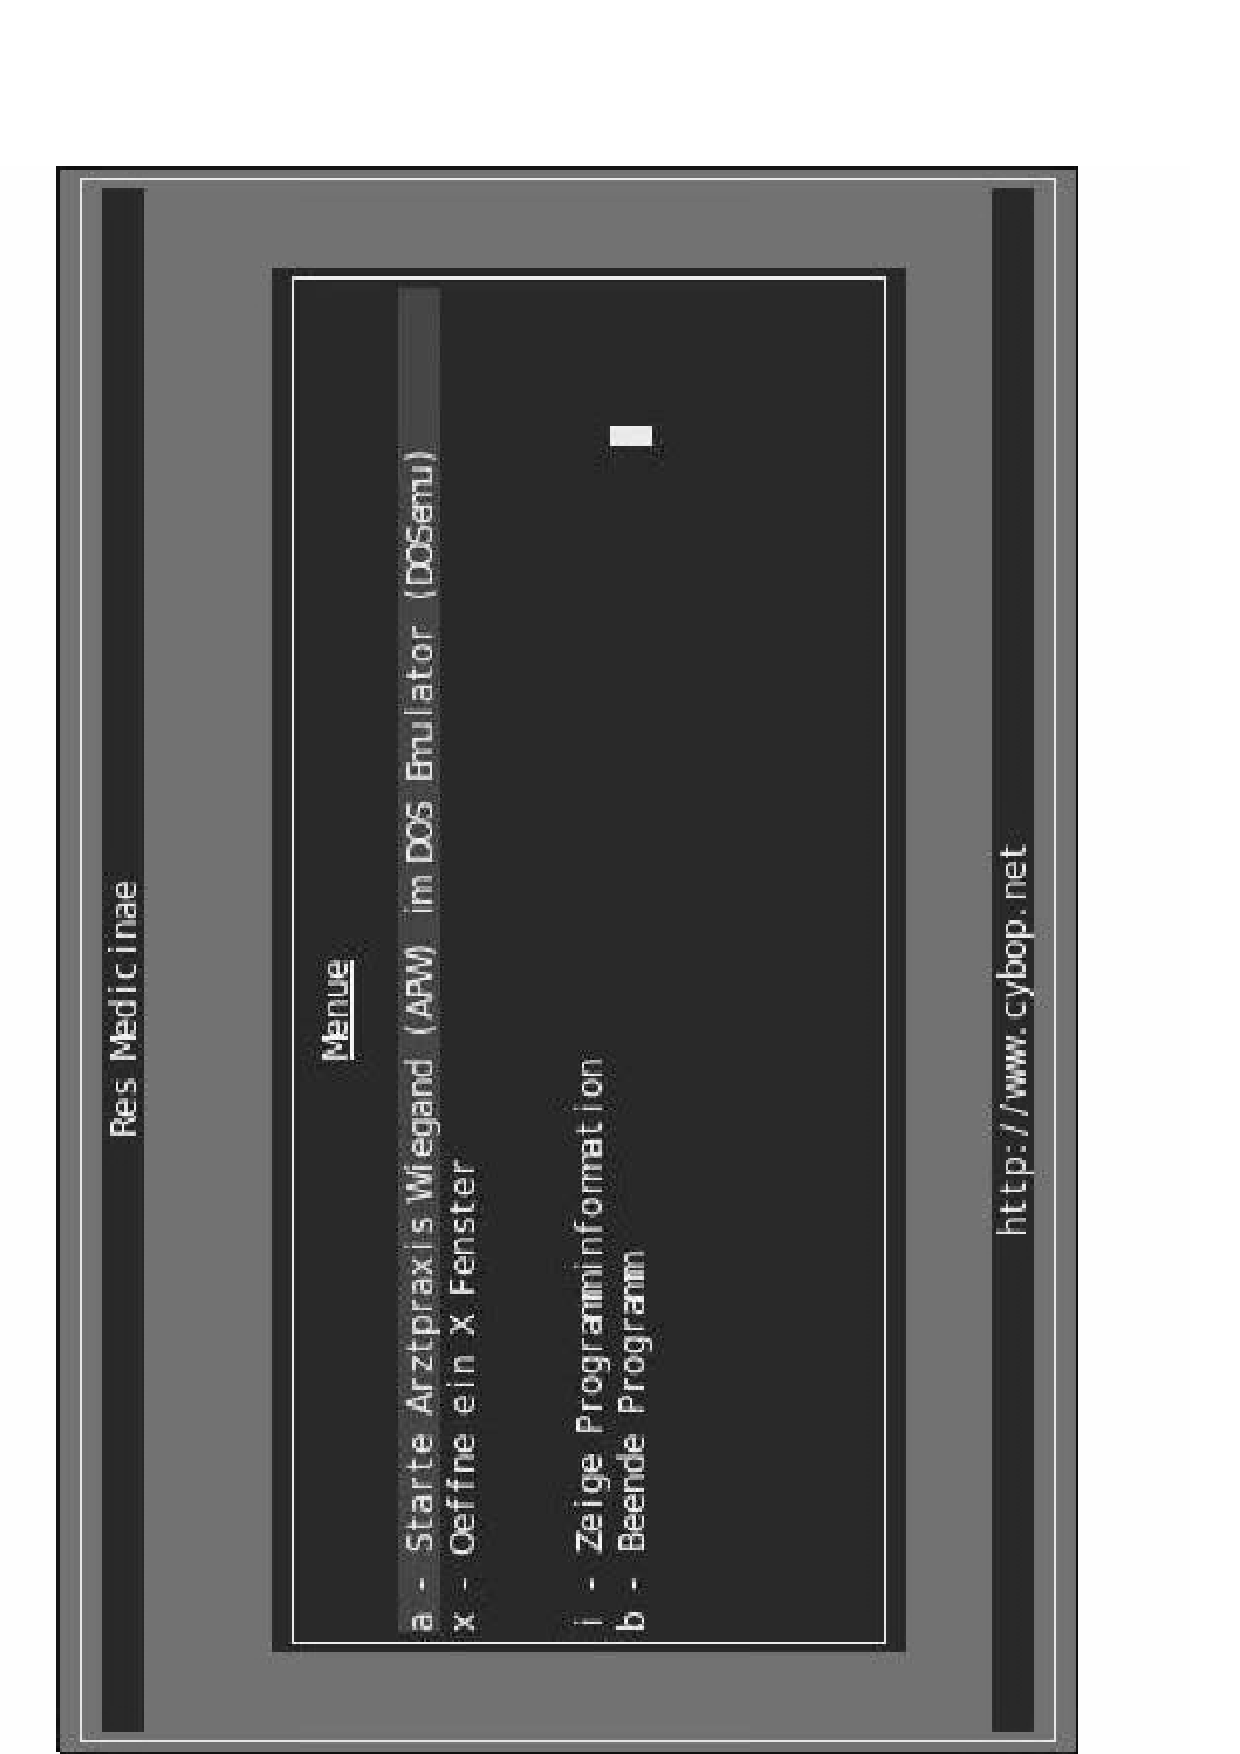
\includegraphics[scale=0.3,angle=-90]{graphics/textual_user_interface.pdf}
        \caption{Textual User Interface}
        \label{textual_user_interface_figure}
    \end{center}
\end{figure}

\subsubsection{Example}

\begin{scriptsize}
    \begin{verbatim}
<part name="exit_menu_item" channel="inline" abstraction="character" model="Exit">
    <property name="position" channel="inline" abstraction="integer" model="5,10,0"/>
    <property name="size" channel="inline" abstraction="integer" model="60,1,1"/>
    <property name="background" channel="inline" abstraction="character" model="blue"/>
    <property name="foreground" channel="inline" abstraction="character" model="white"/>
    <property name="bold" channel="inline" abstraction="boolean" model="true"/>
    <property name="enter" channel="inline" abstraction="knowledge" model=".app.logic.enter"/>
    <property name="previous" channel="inline" abstraction="knowledge" model=".app.tui.about_menu_item"/>
    <property name="next" channel="inline" abstraction="knowledge" model=".app.tui.start_menu_item"/>
    <property name="arrow_up" channel="inline" abstraction="knowledge" model=".app.logic.arrow_up"/>
    <property name="arrow_down" channel="inline" abstraction="knowledge" model=".app.logic.arrow_down"/>
</part>
    \end{verbatim}
\end{scriptsize}

\subsubsection{Position Property}

This property specifies the TUI element's origin.

\emph{required}

name=\texttt{'position'}\\
abstraction=\texttt{'integer'}\\
model=\texttt{x, y, z coordinates}

\subsubsection{Size Property}

This property specifies the TUI element's extension.

\emph{required}

name=\texttt{'size'}\\
abstraction=\texttt{'integer'}\\
model=\texttt{x, y, z extensions}

\subsubsection{Background Property}

This property specifies the background colour of the TUI.

\emph{required}

name=\texttt{'background'}\\
abstraction=\texttt{'character'}\\
model=\texttt{'black' \vline\ 'red' \vline\ 'green' \vline\ 'yellow' \vline\ 'blue' \vline\ 'magenta' \vline\ 'cobalt' \vline\ 'white'}

\subsubsection{Foreground Property}

This property specifies the foreground colour of the TUI.

\emph{required}

name=\texttt{'foreground'}\\
abstraction=\texttt{'character'}\\
model=\texttt{'black' \vline\ 'red' \vline\ 'green' \vline\ 'yellow' \vline\ 'blue' \vline\ 'magenta' \vline\ 'cobalt' \vline\ 'white'}

\subsubsection{Border Property}

This property specifies the kind of border of the TUI.

\emph{optional}

name=\texttt{'border'}\\
abstraction=\texttt{'character'}\\
model=\texttt{'line' \vline\ 'round\_line' \vline\ 'double\_line'}

\subsubsection{Hidden Property}

This property specifies whether or not to hide the TUI element.

\emph{optional}

name=\texttt{'hidden'}\\
abstraction=\texttt{'boolean'}\\
model=\texttt{'true' \vline\ 'false'}

\subsubsection{Inverse Property}

This property specifies whether or not to display the TUI element in inverse
colours.

\emph{optional}

name=\texttt{'inverse'}\\
abstraction=\texttt{'boolean'}\\
model=\texttt{'true' \vline\ 'false'}

\subsubsection{Blink Property}

This property specifies whether or not the TUI element should blink.

\emph{optional}

name=\texttt{'blink'}\\
abstraction=\texttt{'boolean'}\\
model=\texttt{'true' \vline\ 'false'}

\subsubsection{Underline Property}

This property specifies whether or not to underline the TUI element's text.

\emph{optional}

name=\texttt{'underline'}\\
abstraction=\texttt{'boolean'}\\
model=\texttt{'true' \vline\ 'false'}

\subsubsection{Bold Property}

This property specifies whether or not to display the TUI element's text in
bold font.

\emph{optional}

name=\texttt{'bold'}\\
abstraction=\texttt{'boolean'}\\
model=\texttt{'true' \vline\ 'false'}

\subsubsection{Focus Property}

This property points to the TUI element (knowledge model) having focus. It is
important to find out which TUI element a key press event relates to. The focus
of a number of part elements should always be held by their corresponding
whole (compound) element.

\emph{optional}, only if TUI element should be able to react to button press events

name=\texttt{'focus'}\\
abstraction=\texttt{'knowledge' \vline\ 'encapsulated'}\\
model=\texttt{logic knowledge model}

\subsubsection{Previous Property}

This property points to the previous TUI element (knowledge model) owning focus.

\emph{optional}, only if TUI element should have a predecessor that may own the focus

name=\texttt{'previous'}\\
abstraction=\texttt{'knowledge' \vline\ 'encapsulated'}\\
model=\texttt{logic knowledge model}

\subsubsection{Next Property}

This property points to the next TUI element (knowledge model) receiving focus.

\emph{optional}, only if TUI element should have a successor that may own the focus

name=\texttt{'next'}\\
abstraction=\texttt{'knowledge' \vline\ 'encapsulated'}\\
model=\texttt{logic knowledge model}

\subsubsection{Enter Property}

This property specifies the logic knowledge model to be executed if the
\emph{Enter} button is pressed while the TUI element has focus.

\emph{optional}, only if TUI element should react to button press event;
a prerequisition is that the TUI element's \emph{focus} property value is \emph{true}

name=\texttt{'enter'}\\
abstraction=\texttt{'knowledge' \vline\ 'encapsulated'}\\
model=\texttt{logic knowledge model}

\subsubsection{Escape Property}

This property specifies the logic knowledge model to be executed if the
\emph{Esc} button is pressed while the TUI element has focus.

\emph{optional}, only if TUI element should react to button press event;
a prerequisition is that the TUI element's \emph{focus} property value is \emph{true}

name=\texttt{'escape'}\\
abstraction=\texttt{'knowledge' \vline\ 'encapsulated'}\\
model=\texttt{logic knowledge model}

\subsubsection{Arrow Up Property}

This property specifies the logic knowledge model to be executed if the
\emph{arrow-up} button is pressed while the TUI element has focus.

\emph{optional}, only if TUI element should react to button press event;
a prerequisition is that the TUI element's \emph{focus} property value is \emph{true}

name=\texttt{'arrow\_up'}\\
abstraction=\texttt{'knowledge' \vline\ 'encapsulated'}\\
model=\texttt{logic knowledge model}

\subsubsection{Arrow Down Property}

This property specifies the logic knowledge model to be executed if the
\emph{arrow-down} button is pressed while the TUI element has focus.

\emph{optional}, only if TUI element should react to button press event;
a prerequisition is that the TUI element's \emph{focus} property value is \emph{true}

name=\texttt{'arrow\_down'}\\
abstraction=\texttt{'knowledge' \vline\ 'encapsulated'}\\
model=\texttt{logic knowledge model}

\subsubsection{Arrow Left Property}

This property specifies the logic knowledge model to be executed if the
\emph{arrow-left} button is pressed while the TUI element has focus.

\emph{optional}, only if TUI element should react to button press event;
a prerequisition is that the TUI element's \emph{focus} property value is \emph{true}

name=\texttt{'arrow\_left'}\\
abstraction=\texttt{'knowledge' \vline\ 'encapsulated'}\\
model=\texttt{logic knowledge model}

\subsubsection{Arrow Right Property}

This property specifies the logic knowledge model to be executed if the
\emph{arrow-right} button is pressed while the TUI element has focus.

\emph{optional}, only if TUI element should react to button press event;
a prerequisition is that the TUI element's \emph{focus} property value is \emph{true}

name=\texttt{'arrow\_right'}\\
abstraction=\texttt{'knowledge' \vline\ 'encapsulated'}\\
model=\texttt{logic knowledge model}
